% ch2p15_003: Understand ++ prefix for a coordinate
\documentclass[tikz, border=10pt]{standalone}

\usepackage{tikz}

\begin{document}
	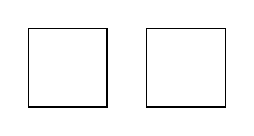
\begin{tikzpicture}
		% Explanation
		% Consider: (x0, y0) -- ++(x1, y1) -- ++(x2, y2)
		%     % (s1_x, s1_y) = (x0 + x1, y0 + y1)
		%     => (s1_x, s1_y) -- ++(x2, y2)
		%     % (s2_x, s2_y) = (s1_x + x2, s1_y + y2)
		
		% So, the coordinate prefixed with ++ will become the new reference for the following coordinate.
		
		
		\def\rectanglepath{-- ++(1cm, 0cm) -- ++(0cm, 1cm) -- ++(-1cm, 0cm) -- cycle}
		
		\draw (0, 0) \rectanglepath;
		\draw (1.5, 0) \rectanglepath;
	\end{tikzpicture}
\end{document}